\chapter{Amostra e Dados Observacionais}
%\addcontentsline{toc}{chapter}{Metodologia}

Conforme apresentado no Capítulo 3, os objetos analisados representam uma amostra de 125 galáxias, sendo 52 com linhas de absorção e 73 com linhas de emissão. Os espectros apresentados (i.e., disponíveis na literatura) foram extraídos do catálogo 6dFGS \cite{jones20046df} e aquelas observadas no OPD/LNA-MCTIC (18 galáxias) serão usadas como controle. Os dados fotométricos foram obtidos de diversas fontes e incluem diferentes bandas espectrais: SDSS (B), 2MASS (vermelho, J; poeira, K), WISE (infra-vermelho, 3.4 e 22$\mu$m), e GALEX (ultravioleta próximo). Uma compilação dessas informações podem ser vistas nos Apêndice B (espectros de absorção) e C (espectros de emissão), respectivamente.


\section{Base de Dados 6dFGS (Six-degree-Field Galaxy Survey)}

Para a análise visual dos espectros e levantamento estatístico dos dados, usamos os espectros da base 6dF Galaxy Survey (6dFGS), \cite{jones20046df}. Trata-se de um levantamento espectroscópico do polo sul galáctico que visa fornecer  posições e velocidades de galáxias situadas do Universo próximo. Quando completo, a pesquisa fornecerá aproximadamente 170\,000 redshifts e 15\,000 velocidades peculiares. A pesquisa utiliza o telescópio britânico Schmidt do Anglo Australian Observatory (AAO), o qual usa o posicionador de fibra robótica 6dF e o sistema de espectrografia. Até o presente momento, é o maior levantamento em redshift do Universo local e de velocidades peculiares. Quando completo, irá abranger todo o céu do sul em torno de um redshift médio de z = 0,05. A Figura 19 ilustra a distribuição desses objetos em coordenadas galácticas.

\begin{figure}[!htbp]
	\centering	
    \caption{}
    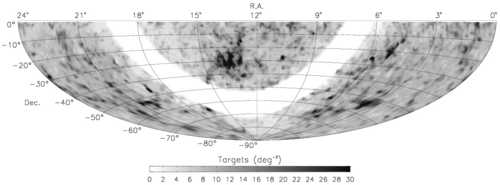
\includegraphics[width=0.8\textwidth]{figuras/6df.jpg}
   	\begin{center}
        \normalsize Fonte: \cite{jarrett2004large} \\Distribuição dos objetos 6dFGS em torno do polo Sul Galático.
    \end{center}
	\label{fig:sbmt-moses}
\end{figure}

Para o polo sul galáctico, tal levantamento se torna importante uma vez que estudos espectroscópicos são escassos para esta região em relação ao norte. Um dos principais catálogos usados para o survey 6dFGS foi o do Two Micron All Sky Survey \cite{jarrett20002mass}.  As principais vantagens para as escolhas de objetos nessas bandas estão diretamente ligadas aos surveys de galáxias no óptico onde a distribuição de energia espectral (SEDs) é predominantemente composto por estrelas azuis jovens, sendo, portanto, fortes indícios de formação estelar recente. Outra razão está ligada ao fato das galáxias do tipo morfológico E/S0 representarem os melhores objetos para fornecer velocidades peculiares do plano fundamental, sendo a maior parcela de galáxia no infravermelho próximo selecionadas. Por fim, uma outra importante vantagem mostra que os efeitos da extinção de poeira são mínimos nos comprimentos de onda do infravermelho.

Um importante objetivo do 6dFGS, denominado "v-survey", consiste em obter dados homogêneos de velocidade-distância para análise das velocidades peculiares. De maneira abreviada, as velocidades relativas das galáxias no Universo possuem, além da componente associada à expansão, outra componente associada aos movimentos peculiares: v = H$_{0}$D + v$_{pec}$. As velocidades peculiares são produzidas pelos campos gravitacionais locais que, por sua vez, se originam das flutuações de densidade locais. O catálogo Mark III contendo tais dados pode ser encontrado em \cite{willick1997homogeneous}.

O acesso aos dados foi feito mediante a submissão de uma tabela CSV com as posições dos objetos (ascensão reta e declinação, J2000.0) da Categoria 7 (objetos de estudo da presente pesquisa) do catalogo de Arp \& Madore \cite{arp1987catalogue} na base de dados no site do 6dFGS \cite{jones20096df} utilizando o serviço “Xmatch form”. Uma vez submetido, o retorno da tarefa oferece acesso aos espectros e as imagens referentes com as bandas JHK do 2MASS e B e R do UKST (United Kingdom Schmidt Telescope). Um script em Python também foi feito para automatizar o download dos objetos escolhidos. Isso se deve ao fato do site 6dFGS fornecer o descarregamento de apenas um objeto por vez.

Foram encontrados 125 espectros na base de dados 6dFGS, referentes a 225 objetos presentes na Categoria 7. Com esses objetos em mãos e com os programas feitos na linguagem Python, foi possível analisar visualmente como os objetos se comportam nas diversas bandas em relação aos espectros. Para este primeiro momento, tal análise é importante pois tornar possível a separação quanto a atividade nuclear e o julgamento para caracterizar se os jatos e as galáxias associadas podem (ou não) pertencer a esta Categoria (ou serem migrados para a Categoria 15).

\section{Identificação das Linhas de Emissão}

A criação de um script que faça a distinção espectral entre galáxias normais e ativas (regiões HII ou Starburst e AGN - Active Galactic Nuclei - Seyfert e LINER (Low Ionization Nuclear Emission-line Region), seguem parâmetros simples que levam apenas em consideração informações específicas contidas no cabeçalho (header) das imagens FITS. Nele está presente informações como tempo de exposição, época de observação, posição do objeto, informações do espectro, dentre outros. As informações necessárias para a escrita do script se referem ao elemento de partida e valor de incremento do comprimento de onda. Com essas informações obtidas no cabeçalho, foi possível criar uma cópia do espectro para assim modelar e analisar cada valor em particular. O acesso aos elementos nos arquivos FITS do survey 6dFGS ocorre de forma simples, buscando os valores CRVAL1 e CDELT1 que correspondem ao valor de partida e incremento como descrito acima. Tendo em vista que a coluna referente ao comprimento de onda (\AA) não pode ser acessado, coube gerar então a coluna que o corresponda utilizando as informações CRVAL1 e CDELT1 e então analisá-lo paralelamente junto a coluna do fluxo. Uma vez criado o modelo do espectro, coube delimitar de maneira eficiente a região referente do comprimento de onda a ser calculado. Para isso, subtrai-se do valor inicial do comprimento de onda (CRVAL1) o valor 6560 \AA, que correspondente ao limite da região e o começo da região equivalente a linha de emissão H$\alpha$. Tendo em vista que para cada espectro o valor de incremento é diferente no comprimento de onda, pois cada galáxia possui um redshift diferente, dividi-se o valor obtido anteriormente pelo CDELT1, evitando assim flutuações nos valores delimitantes definidos. Sendo assim os valores serão sempre exatos para quaisquer espectro usado. Identificada a região do H$\alpha$, usamos o valor final mencionado anteriormente como o valor inicial para esta região. Quanto ao valor final, estimamos cinco pixels como média de término da gaussiana. De posse dos valores, o próximo passo foi comparar se o valor médio da primeira região é menor que a região do H$\alpha$. 

O método utilizado emprega uma medida direta de comparação da média do fluxo e a média da região onde possivelmente existe a linha de emissão do H$\alpha$. O método utilizado a priori obteve uma pequena margem de erro ($<$ 2\%), uma vez que analisamos apenas a linha de emissão do H$\alpha$ (com fraca intensidade em alguns casos), a qual normalmente caracteriza uma galáxia com atividade nuclear. Uma simples verificação visual resolve o problema.

Após as comparações, os arquivos FITS são então separados em duas pastas com seus respectivos tipos, normais e ativas. Este código pode ser empregado para qualquer espectro 1d, sendo necessário apenas a mudança da região a ser estudada. Contudo, é importante salientar que existe uma pequena margem de erro, a qual depende da intensidade da linha escolhida. As razões para os erros estão relacionadas a vários fatores, mas, sobretudo, ao valor da razão sinal-ruído do espectro estudado, na qual depende, dentre outros fatores, da sensibilidade do detector CCD empregado na observação e das condições do sítio observacional.

\section{Imagens Multibandas}
\label{subsec:image_mult}

Obter e analisar visualmente as imagens dos objetos estudados nas diversas bandas, representa uma tarefa fundamental para o nosso estudo, uma vez que estamos interessados em caracterizar a peculiaridade da Categoria 7: os jatos. Com esta finalidade, um programa Python foi escrito para criar para cada objeto de estudo uma figura com seis imagens contendo as bandas DSS2 Blue, 2MASS-J, 2MASS-k, WISE 3.4, WISE 22 e GALEX far UV. Tais imagens foram recolhidas através do serviço SkyView \url{(https://skyview.gsfc.nasa.gov/)} que falaremos a seguir.

Através de bibliotecas Python dedicadas a pesquisas astronômicas, é possível acessar, transferir e visualizar as imagens requisitadas no formato FITS. Para este fim, usamos o pacote Astroquery \cite{sipocz2016astroquery}. Astroquery é um pacote filiado da Astropy \cite{robitaille2013astropy}, ou seja, um conjunto de ferramentas para consulta de formulários e banco de dados astronômicos. A Astroquery permite aos usuários acessar dados astronômicos on-line a uma extensa gama de fontes. Cada serviço astronômico da Web possui seu próprio sub-pacote para a interface com uma fonte de dados específica. 

Para o acesso das imagens dos objetos, usamos o SkyView que oferece um serviço de recorte para uma série de consulta de imagens. Existem dois métodos principais para o uso do serviço: \textit{get\_images}, que faz a busca e realiza o download do arquivo, enquanto o  \textit{get\_image\_list} apenas procura pelo arquivo e retorna uma lista de resultados. Usamos o primeiro método, \textit{get\_images}, pois após o descarregamento ainda será necessário submetê-lo as tarefas seguintes do programa. Estão disponíveis em ambos os métodos alguns parâmetros onde é possível entrar com as configurações do objeto a ser acessado. A função principal escrita para o programa possui os seguintes parâmetros:

\begin{itemize}

\item Position: Determina o centro do campo para ser  recuperado. Este parâmetro dá suporte as coordenadas, e os nomes dos objetos são convertidos em coordenadas através do resolvedor de nomes do bancos de dados, SIMBAD \url{(simbad.u-strasbg.fr/)} ou NED \url{(https://ned.ipac.caltech.edu/)}. Ambas entradas devem ser do tipo "string". Usamos como entrada as coordenadas presentes no arquivo CSV através da função SkyCoord no formato equatorial e já convertidas para a época padrão J2000.0 através do serviço de conversão do Vizier \url{ (vizier.u-strasbg.fr/viz-bin/VizieR)}, uma vez que o catálogo de Arp \& Madore estão posicionados para J1950.0;

\item SkyCoord: Essa função é usada como ferramenta auxiliar na entrada das coordenadas para a função "Position", pois fornece uma interface flexível para a manipulação e transformação de coordenadas celestes. Através dele, é possível a submissão de uma ou mais coordenadas que podem ser listas, duplas e arrays, produzindo coordenadas escalares ou de matrizes. Na função Skycoord usamos também alguns parâmetros disponíveis necessários:
\item Frame: Este é o tipo de coordenada que o SkyCoord deve representar. Usamos o Sistema Internacional de Referência Celeste (ICRS, na sigla em inglês) como padrão;
\item Unit: Unidades para os valores LAT e LON (coordenadas geográficas), recuperadas anteriormente; Obstime faz referência à data de observação;
 
\item Survey: Lista dos surveys de interesse;
\item Pixels: Aqui passamos as dimensões em pixels da imagem a ser produzida. Usamos o padrão 300 x 300. O sistema de coordenada escolhido é o equatorial J2000.0.
\end{itemize}

Como usamos apenas as imagens como forma de comparação visual, atribuímos aos parâmetros "grid" e "gridlabels" o valor "False", pois não se faz necessário neste caso. Para produzir uma imagem para cada banda, chamamos a mesma função com as mesmas configurações, exceto o parâmetro "survey", onde usamos para cada imagem criada uma entrada diferente.

Usamos as bibliotecas do Matplot como Subplot2grid para cuidar da plotagem de forma dinâmica. A vantagem para seu uso se dá pela fácil manipulação. Sendo assim a customização e criação de subplots é feita de forma mais eficiente e de melhor manutenção para revisões e estudos futuros. Após as transferências, os plots gerados com o Subplot2grid são salvos como imagens em uma pasta previamente criada através do programa para este fim. Um exemplo é ilustrado na Figura 4.2.

\begin{figure}[H]
	\centering	
    \caption{AM 0222-250}
    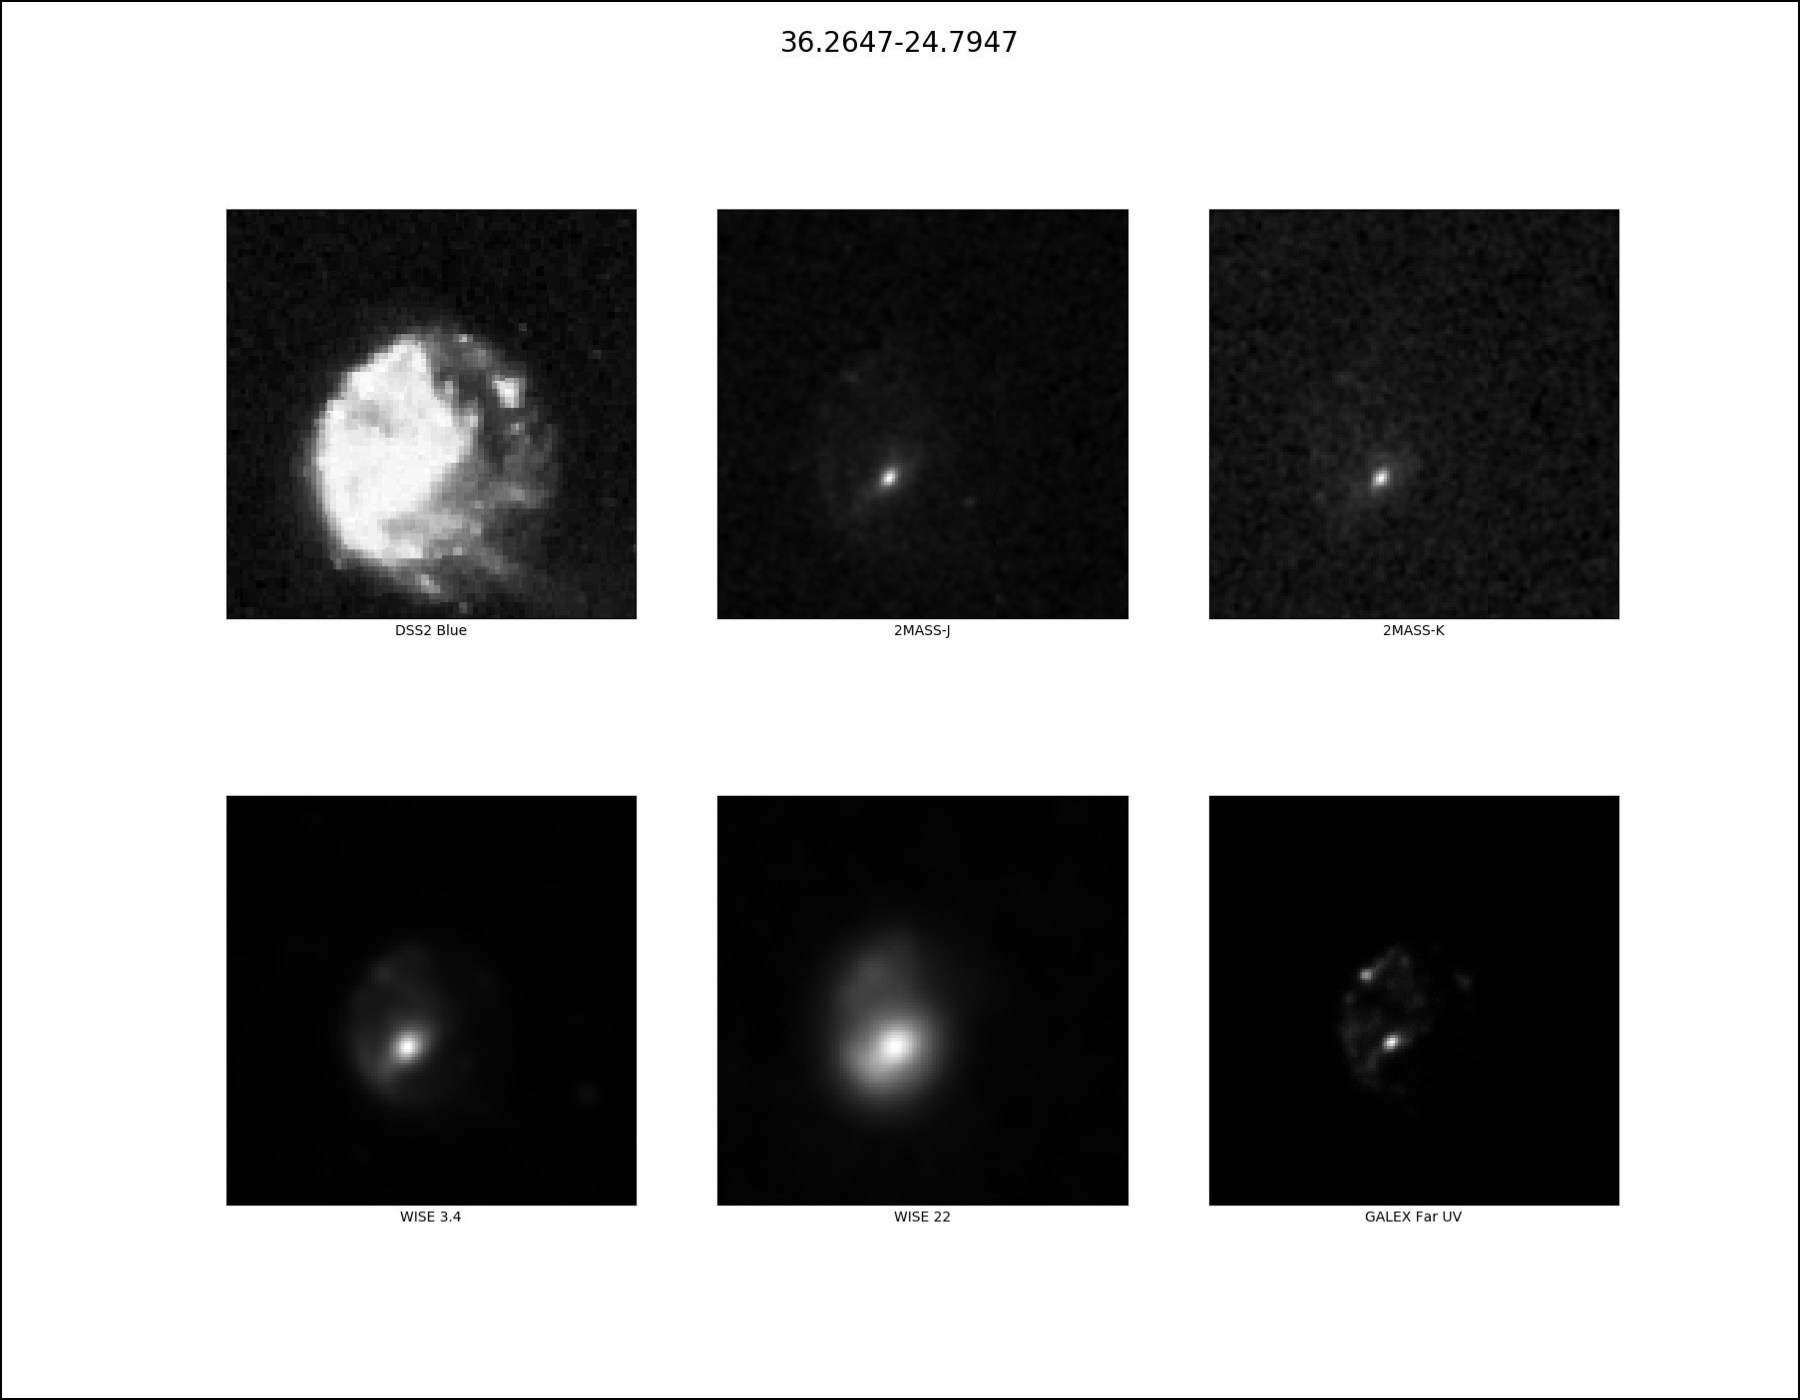
\includegraphics[width=0.6\textwidth]{figuras/AM-0222-250.png}
   	\begin{center}
        \normalsize Fonte: Próprio Autor \\Imagem gerada das diversas bandas da galáxia AM 0222-250
    \end{center}
	\label{fig:fotometry_mosaic}
\end{figure}

\section{Espectros e Multibandas}
\label{subsec:spec_mult}
Em adição aos programas anteriores, um outro programa foi escrito visando mostrar, em conjunto com as imagens nas bandas fotométricas, os espectros disponíveis da base 6dFGS. Um dos objetivos para a geração das imagens em conjunto com os  espectros é justificado pela relação que as galáxias possuem com os diferentes filtros observados. Parte do código segue a metodologia descrita acima para gerar as imagens. Uma vez que os surveys são acessados através das coordenadas do arquivo em CSV, o algoritmo compara como números inteiros as posições RA e DEC com as posições encontradas no cabeçalho do arquivo FITS. Esse método se torna necessário pois as conversões feitas pelo Vizier para a época J2000.0 não estão totalmente calibradas, tendo uma pequena diferença nos números flutuantes. Tal comparação obteve sucesso, uma vez que a quantidade de posições presentes no catálogo é relativamente pequena, não havendo semelhança entre eles. 

Gerar as imagens dos espectros segue também parte do método empregado na identificação das galáxias ativas. Usamos as informações contidas nos ``headers`` dos arquivos FITS onde contém o valor CRVAL1 e CDELT1 que corresponde a  partida do fluxo e do incremento,  respectivamente. Acessamos também as colunas correspondentes  ao fluxo de cada espectro. Os espectros gerados em nada diferem do original, tendo em vista que cada pixel é reproduzido fielmente seguindo os requisitos descritos anteriormente.

Para facilitar a identificação das principais linhas de emissão nas bandas do visível e do infravermelho próximo, foram feitas marcações nas áreas já conhecidas da primeira coluna correspondente ao comprimento de onda, tal como feita na marcação da linha do H$\alpha$. Cada área marcada corresponde ao começo e o fim de cada gaussiana. Uma vez marcada as áreas de interesse, restou definir em uma variável cada valor máximo de cada área. Por conseguinte, na função de plotagem \textit{subplot2grid} definimos no parâmetro \textit{annotate}, as variáveis que contém os valores máximos de cada linha de emissão extraídos de cada fluxo para então marcar tal linha com a determinada identificação química.

De posse dessas informações integradas, imagens e espectros, concluímos então a nossa amostragem de estudo. A Figura \ref{fig:1146-270} ilustra esse procedimento final. É possível perceber na imagem da banda B do DSS2, a presença de um fino jato a direita do objeto (direção Oeste), provavelmente associado com a componente nuclear que deve ser bastante energética. Por outro lado, as imagens do 2MASS nas bandas J e K apontam, respectivamente, a presença de poucas estrelas velhas e de poeira, porém, sendo mais intensas nas bandas exploradas pelo WISE. Com o GALEX, é possível reconhecer duas subestruturas de altas energias, que podem ser claramente um processo de fusão dos núcleos de duas galáxias, dada a evidência das intensas linhas de emissão no espectro representado. Esse resultado pode ser um importante indício para a presença do jato nesse objeto peculiar.

\begin{figure}[H]
	\centering	
    \caption{AM 1146-270}
    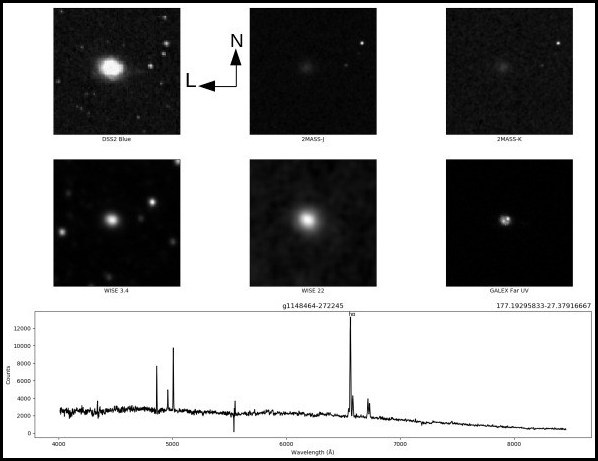
\includegraphics[width=0.8\textwidth]{figuras/g1148464-272245.jpg}
   	\begin{center}
        \normalsize Fonte: Próprio Autor \\Imagens das bandas e do espectro da galáxia peculiar AM 1146-270. A direção Norte está para cima, e a direção Leste para a esquerda.
    \end{center}
	\label{fig:1146-270}
\end{figure}

Embora o resultado obtido acima advindo de uma possível fusão de duas galáxias possa fomentar uma interessante conclusão, é necessário que façamos primeiro uma análise do jato observado na banda B do DSS2. Lembramos que muitos objetos presentes na Categoria 7, definidos por Arp e Madore, podem não conter o jato, sendo, por exemplo, um filamento, cauda, laços de matéria ou detritos (Categoria 15). Alguns métodos são óbvios, mas estão incluídos para garantir a completude deste trabalho.

Um outro aspecto da metodologia está relacionada com a modelagem espectral das galáxias analisadas via o código de síntese espectral STARLIGHT (\cite{cid2004star,fernandes2005semi,asari2007history}), onde esperamos obter alguma conclusão que possa contribuir para a compreensão dessa característica peculiar observada.
